\section{}
The mass is $M = 1$ kg, but the values of the damper $D$ and spring $K$ are unknown. In order to
identify these, a 10 N amplitude step input $u(t) = 10[1_{+}(t)]$ is applied to the system initially at rest.
The resulting (underdamped) response $y(t)$ is plotted below, showing the peak and steady-state
values:
\begin{figure}[h]
    \centering
    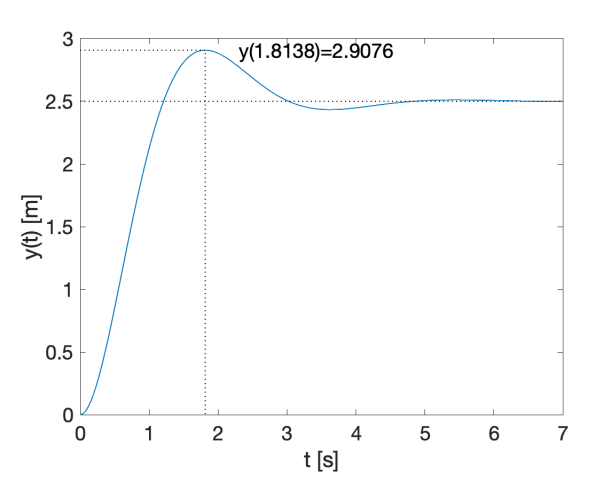
\includegraphics[width=0.9\textwidth]{Questions/Figures/Q2ProblemDiagram.png}
    \caption{Second-order system response to a unit step input with annotations}
    \label{fig:Q2ProblemDiagram}
\end{figure}

\subsection{}
Calculate the values of $\zeta$ and $\omega_n$ for this system \\

\textbf{Solution} \\

The transfer function of this system, as given in the notes (p. 53) is:
\begin{align}
    G(s) &= \frac{1/M}{s^2 + 2 \zeta \omega_n s + \omega_n^2} \nonumber \\
    \omega_n &= \sqrt{\frac{K}{M}} \label{eq:omega_n} \\
    \zeta &= \frac{D}{2 \sqrt{MK}} \label{eq:zeta}
\end{align}

Converting the transfer function to standard form, we get:
\begin{align*}
    G(s) &= \frac{1}{K} \frac{\omega_n^2}{s^2 + 2 \zeta \omega_n s + \omega_n^2} \\
\end{align*}

The response is:
\begin{align*}
    Y(s) = \underbrace{\frac{10}{K}}_{\alpha} \frac{\omega_n^2}{s(s^2 + 2 \zeta \omega_n s + \omega_n^2)}
\end{align*}

For a standard second-order system (p. 59),
\begin{align*}
    \omega_n &= \frac{2 \pi}{t_p \sqrt{1 - \zeta^2}} \\
    \zeta &= \sqrt{\frac{\ln^2(M_p))}{\pi^2 + \ln^2(M_p)}}
\end{align*}

From the graph, we see that $t_p = 1.8138$,
$y(t_p) = 2.9076$, and $y_{\infty} = 2.5$.
\begin{align*}
    M_p &= \frac{y(t_p) - y_{\infty}}{y_{\infty}} \\
    &= \frac{2.9076 - 2.5}{2.5} \\
    &= 0.16304
\end{align*}

\begin{empheq}[box=\fbox]{align*}
    \zeta &= \sqrt{\frac{\ln^2(0.16304)}{\pi^2 + \ln^2(0.16304)}} \\
    &= 0.4999918 \approx 0.5 \\
    \omega_n &= \frac{2 \pi}{1.8138 \sqrt{1 - 0.5^2}} \\
    &= 3.99999859794 \approx 4
\end{empheq}

\subsection{}
Using the information from (a), find the values of $D$ and $K$

\textbf{Solution}
From Eq. (\ref{eq:omega_n}),
\begin{align*}
    K &= M \omega_n^2 \\
    &= 1 \cdot 4^2 \\
    &= \boxed{16}
\end{align*}

From Eq. (\ref{eq:zeta}),
\begin{align*}
    D &= 2 \sqrt{MK} \zeta \\
    &= 2 \sqrt{1 \cdot 16} \cdot 0.5 \\
    &= \boxed{4}
\end{align*}  